\documentclass[a4paper]{article}

\setlength{\oddsidemargin}{-1in}
\addtolength{\oddsidemargin}{0.05 \paperwidth}
\setlength{\evensidemargin}{-1in}
\addtolength{\evensidemargin}{0.05 \paperwidth}
\setlength{\textwidth}{0.9 \paperwidth}

\setlength{\topmargin}{-0.75in}
\addtolength{\topmargin}{0.05 \paperheight}
\setlength{\textheight}{\paperheight}
\setlength{\headheight}{0in}
\setlength{\headsep}{0in}
\setlength{\footskip}{0in}

\setlength{\parskip}{0.3cm}
\setlength{\parindent}{0pt}
	
\usepackage[T1]{fontenc}
\usepackage[utf8]{inputenc}
\usepackage[german]{babel}
\usepackage{eurosym}

\usepackage[default,scale=1.5]{opensans}
\usepackage[scaled=1.4]{beramono}
\linespread{1.7}

\usepackage{url}
\usepackage{graphicx}

\usepackage{booktabs}


\usepackage{color}
\definecolor{freifunkpink}{RGB}{215,0,73}
\definecolor{freifunkyellow}{RGB}{255,191,0}
\definecolor{lightgrey}{RGB}{220,220,220}

\usepackage{enumitem}
\setlist[itemize]{leftmargin=*}

\begin{document}
\thispagestyle{empty}
 
\begin{center}
\Huge \textit{\textbf{\textcolor{freifunkpink}{Internet für Flüchtlinge}}} \\
\vspace{0.6cm}
\large Freifunk ist ein regionales Mitmach-Netz für WLAN und Internet.\\
Hilf uns das Netz in deinem Stadtteil auszubauen \\
und teile dein Internet mit anderen Menschen!
\normalsize

\vspace{1.0cm}
\end{center}

{ \fontfamily{augie}\selectfont{\huge {}Liebe Nachbarn!}}
\vspace{0.5cm}

Freifunk Darmstadt ist eine lokales Projekt mit dem Ziel, in Darmstadt und Umgebung ein \emph{offenes} und \emph{kostenloses} WLAN-Netzwerk aufzubauen. Wir stellen Technik bereit, mit der \emph{jeder} seinen Internetzugang \emph{unkompliziert} mit anderen teilen kann. Das Netz ist so aufgebaut, dass die Risiken für Betreiber minimal sind und das Heimnetz geschützt bleibt.

Die Flüchtlinge, die seit kurzem Eure Nachbarn sind, benötigen einen Internetzugang, um Kontakt mit ihrer Familie und ihrer alten Heimat zu halten. Ein internetfähiges Gerät ist heute auch für Flüchtlinge erschwinglich, jedoch können viele sich die vergleichsweise teuren Datentarife der Mobilfunkanbieter nicht leisten.

Zur Zeit unterstützen schon etwa 170 Menschen in Darmstadt und Umgebung Freifunk und teilen ihren Internetzugang. \emph{In der Nähe der Flüchtlingslager gibt es zur Zeit noch nicht genug Zugangspunkte um eine vollständige Versorgung zu gewährleisten!}

Ihr könnt helfen und selbst einen Router für Freifunk installieren. Eine Liste von geeigneten Geräten haben wir auf der Rückseite zusammengestellt. Für die Installation folge der Anleitung auf unserer Webseite. Wenn es zu Problemen kommt, helfen wir gerne.
Wenn Ihr euch mit der technischen Seite nicht so gut auskennt, könnt Ihr auch ein von uns vorbereitetes Gerät bekommen!

\vspace{0.6cm}

\begin{center}
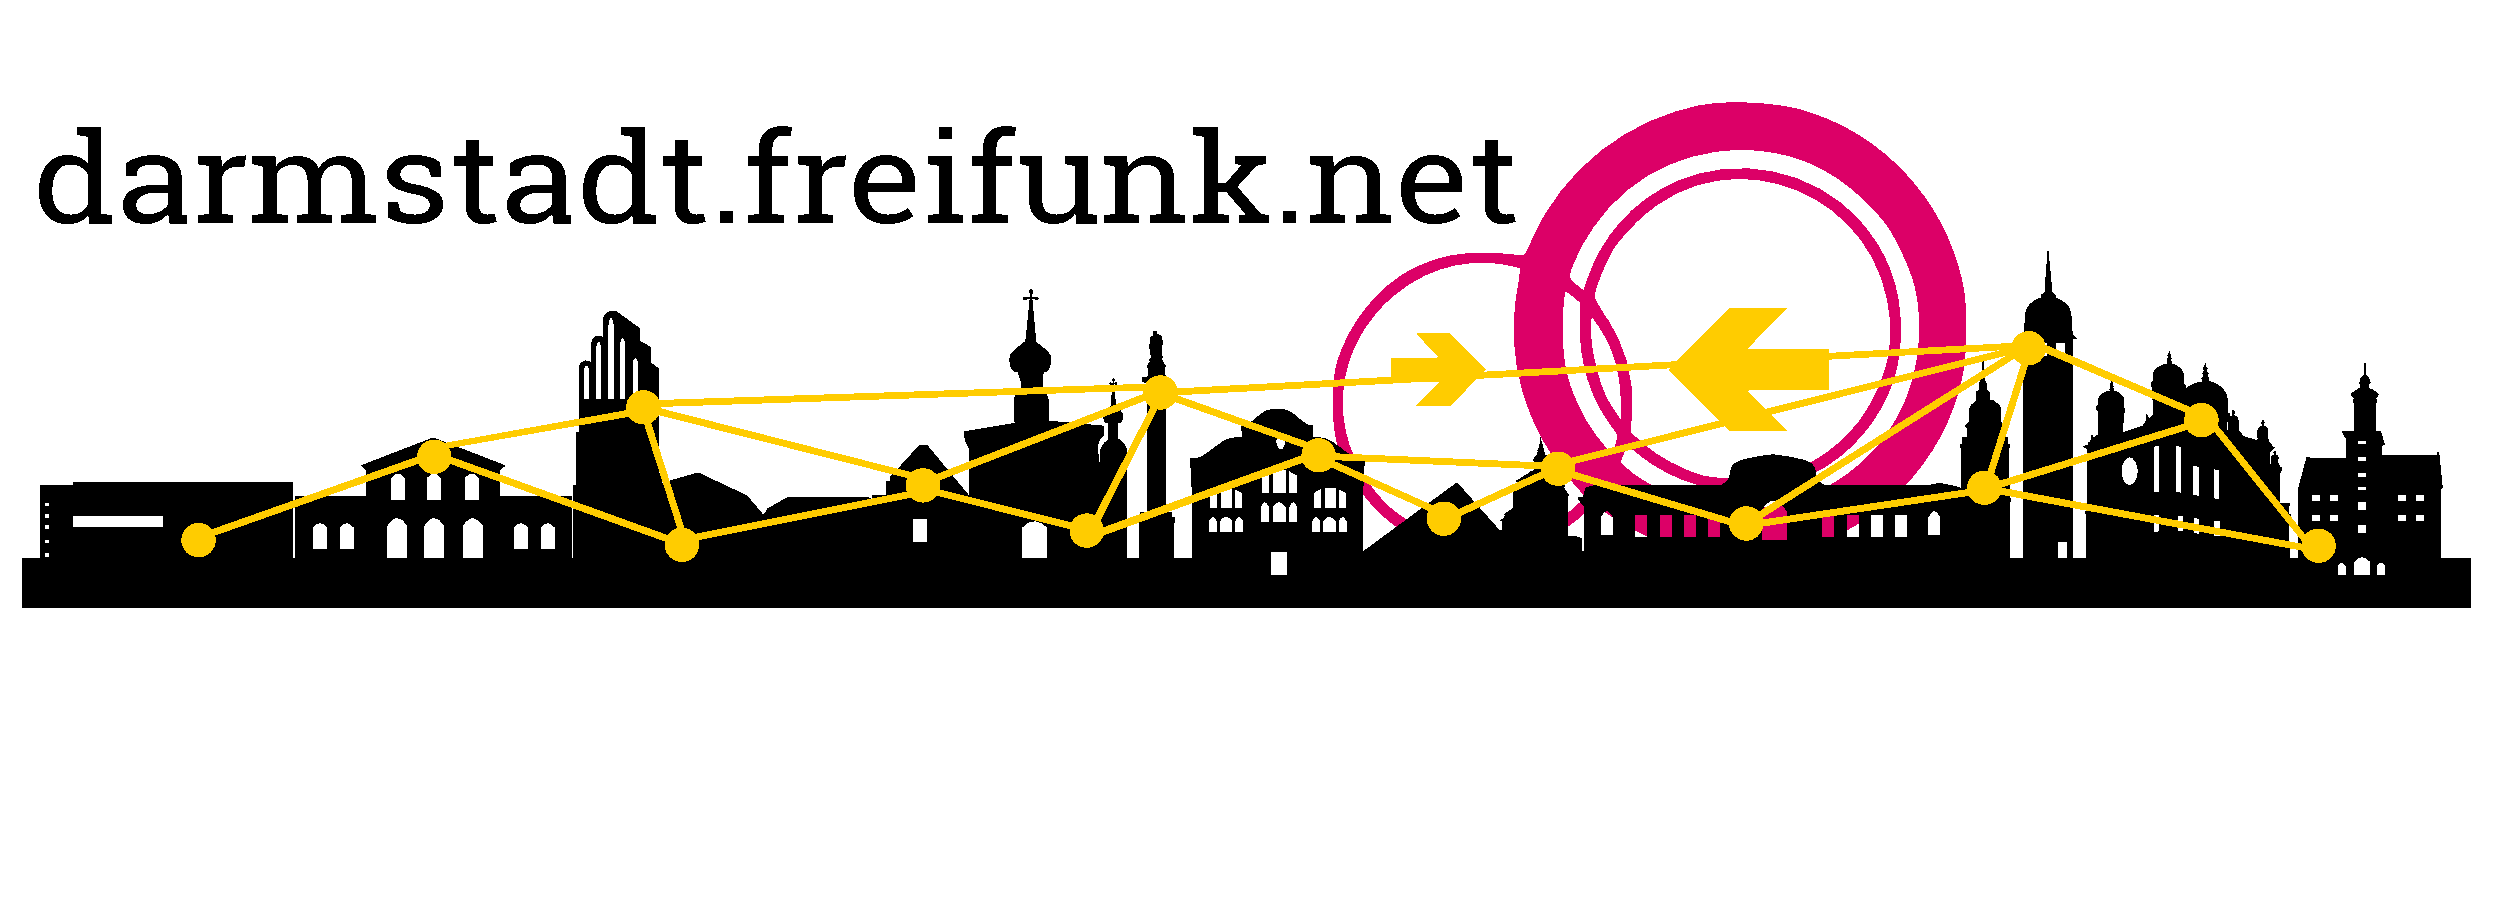
\includegraphics[width=\textwidth]{logo-refugees}
\end{center}

\newpage

\thispagestyle{empty}

\textbf{Unterstützte Geräte}

\begin{center}
\begin{tabular}{lccc} \toprule
	Modell (Herst.: TP-Link) & Preis ca. & WLAN (2,4/5\,GHz) &Freifunk-VPN Datenrate \\ \midrule
	TL-WR842 (N / ND, v2) & \EUR{30} & 300 / -- & bis zu 16 Mbit/s \\
	TL-WR1043 (ND v2, v3) & \EUR{45} & 450 / -- & bis zu 23 Mbit/s \\
	Archer C5 v1.2 & \EUR{75} &300 / 866 & bis zu 23 Mbit/s\\
	Archer C7 v2 & \EUR{95} & 450 / 1200 & bis zu 23 Mbit/s\\	
	\bottomrule
\end{tabular}
\end{center}

Die meisten Geräte sind online bei z.\,B. Amazon oder in Darmstadt bei Zimmermann Elektronic  (Kreuzung Rhein-/Neckerstraße) oder Saturn (Fussgängerzone Innenstadt oder Loop5) erhältlich. Alternativ könnt Ihr auch für das Projekt spenden, damit wir selbst mehr Zugangspunkte aufbauen können. \\
\textbf{Spendenseite:} https://darmstadt.freifunk.net/mitmachen/spenden
\begin{center}
\vspace{.3cm}
\hspace*{-0.05 \paperwidth}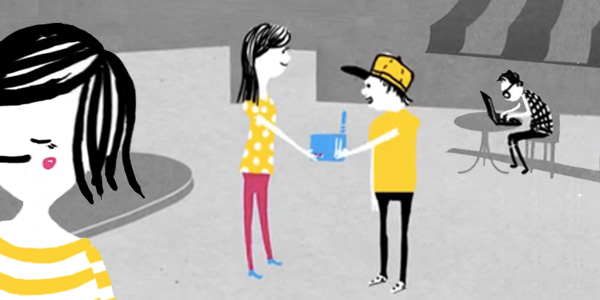
\includegraphics[width=\paperwidth]{community}
\vspace{.3cm}
\end{center}

Alle Informationen \& Kontakte findet Ihr auf \textbf{http://darmstadt.freifunk.net}. Bei Fragen schreibt uns eine Mail an \textbf{info@darmstadt.freifunk.net}.

Unser \textbf{offenes Treffen} findet \emph{jede Woche Montags um 19:00 Uhr} in der Willhelm-Leuschner-Straße 36 (Im Hinterhof), Darmstadt statt. Ihr seid herzlich eingeladen!


\end{document}
